\documentclass[12pt, letterpaper, twoside]{article}
\usepackage[utf8]{inputenc}
\usepackage[english]{babel}
\setcounter{secnumdepth}{3} % default value for 'report' class is "2"
% Bib & space between bib entries
\usepackage{natbib}   
\setlength{\bibsep}{0pt plus 0.3ex}

% Space between lists
\usepackage{enumitem}
\setlist{nolistsep}
\nocite{*}
% Force figures to stay in place
\usepackage{float}

% Image
\usepackage{graphicx}
%\graphicspath{ {..09_figures/} }
%\setlength{\parindent}{2em}
%\setlength{\parskip}{1em}

\renewcommand{\thesubsubsection}{}

\usepackage{hyperref}
\hypersetup{
    colorlinks=true,
    linkcolor=blue,
    filecolor=magenta,      
    urlcolor=cyan,
    citecolor=black
}

\urlstyle{same}
\usepackage{geometry}
\geometry{letterpaper, margin=1in}

\usepackage{sectsty}
\sectionfont{\normalsize}
\subsectionfont{\normalsize}
\subsubsectionfont{\normalsize}

% To remove section numbering
%\setcounter{secnumdepth}{0}

\usepackage{titlesec}
%\titlespacing{\section}{0pt}{\parskip}{-\parskip}
%\titlespacing{\subsection}{0pt}{\parskip}{-\parskip}
%\titlespacing{\subsubsection}{0pt}{\parskip}{-\parskip}
\titlespacing\section{0pt}{12pt plus 2pt minus 2pt}{0pt plus 2pt minus 2pt}
\titlespacing\subsection{0pt}{12pt plus 2pt minus 2pt}{0pt plus 2pt minus 2pt}
\titlespacing\subsubsection{0pt}{12pt plus 2pt minus 2pt}{0pt plus 2pt minus 2pt}




\titlespacing{\subsection}{\parindent}{.5ex}{.5em}
\titlespacing{\subsubsection}{\parindent}{.1ex}{.1em}

\usepackage{amsmath}
\usepackage{setspace}
\doublespacing

\usepackage{subfig}


\begin{document}


\title{%
A Machine Learning Approach to Home Field Advantage in the NFL  \\ 
\large PPOL 564 Final Project \\
\normalsize Word count: 2966}
\author{Chau Nguyen}
\date{\today}
\maketitle


\section{Introduction}

In this project, I want to learn what constitutes ``Home field advantage'' in the National Football League (NFL). Using machine learning techniques and unique game-level data spanning 28 seasons, I aim to answer the question: ``Why do home teams tend to win more?''

The report is organized as followed: Section 2 gives an overview of what home field advantage is, Section 3 discusses the data used, Section 4 explains the analysis, Section 5 lays out the results of my findings, and Section 6 ends with further discussions on the topic. 

\section{Problem Statement and Background}

``Home field advantage'' is often taken for granted in sports analysis - teams are \textit{assumed} to have a competitive edge when playing at their home stadiums. In a meta-analysis across  a variety of sports, game types and error, \cite{hfa1} found that home teams do win more and hypothesized that crowd noise is one the main reasons. As the phenomenal exists across all sports, the NFL is no exception.  According to FiveThirtyEight.com, ``the NFL home field advantage is real'' and ``over 57 percent of games are won by home teams'' \citep{538}. \cite{538}, on the other hand, does not find that crowd noise affects the ``false start''\footnote{After the neutral zone has been established (ball is made or declared ready for play), an offensive player may not make a false start, a defensive player may not encroach (initiate contact with a member of the offensive team) or commit a neutral zone infraction, and no player of either team may be offside when the ball is put in play. \citep{falsestart}} rate for road teams in the league. Similarly, \cite{scorecasting} did not find that crowd noise affects the away team's performance in other sports. 

Then the 2020 covid-19 global pandemic took place. If the NFL wanted to have a season at all, teams needed to adhere to local health guidelines. With stadiums having to limit crowd capacity (or not allow fans in the stands whatsoever), pundits and analysts made bold claims that ``There's no such thing as home-field advantage in the NFL this season'' because ``fans, if any, in the stands means less crowd noise to disrupt the road team's offensive flow'' \citep{wapo}. Contradicting beliefs on what makes ``home field advantage'' what it is does not change analysts' beliefs that the phenomenon exists. 

My theory is that ``home field advantage'' in the NFL is more about what the \textit{away team} has to do in other to play the game than the home team winning. For instance, the Seattle Seahawks, a West Coast team, is scheduled to travel 28,082 miles in 2020, while the Baltimore Ravens, an East Coast team, is only supposed to fly 6,420 miles to get to their games - this is a significant discrepancy \citep{cbs}. I think that the 3-hour difference in time zones from coast-to-coast traveling can also affect a team's performance, and the more a team has to fly, the less time they get to rest. With this project, I aim shed light on what factor affects ``home field advantage'' in the NFL using machine learning. 

\section{Data}

\subsection{Source}
I built several webscrapers using python package BeautifulSoup \citep{soup} to scrape the dataset. Data on stadiums was scraped from \url{Wikipedia.com} and data on team records, game schedule and fan attendance was scraped from \url{Pro-Football-Reference.com} (PFR). 

\subsection{Coverage}
The scraped data from PFR covers 28 NFL seasons from 1992 to 2019, totaling 7292 unique games. 

\subsection{Unit of observation}
The unit of observation is the outcome of each individual game. 

\subsection{Unit of analysis}
Game data is reshaped into a dyadic dataset, with each dyad represents a single game. Each member of the dyad represents the one of the two teams in the game and thus distinguishable from the other.

\subsection{Variables of interest}

\subsubsection{Target variable}
The target variable is a dichotomous variable \textit{Win} which equals 1 if the first team in the dyad (Team\_A) has a positive points differential (which means they have won the game) and equals 0 if the points differential for Team\_A is negative. 

\subsubsection{Feature Variables}
The following variables are used to capture the ''Home field advantage'' of each team::
\begin{itemize}[noitemsep, leftmargin=*]
	
	\item \textit{Time\_rest\_days}: Continuous variable measuring the number of days between two games for Team\_A.
	
	\item \textit{Miles\_traveled}: Continuous variable measuring the distance between the coordinates of Team\_A and Team\_B's home stadiums. This variable was calculated using the Great-Circle distance formula following the methods described by \cite{distance}.
	
	\item \textit{Time\_diff}: Continuous variable measuring the number of hours in timezone between a team's home stadium and the stadium the game is being played at. 
	
	\item \textit{Capacity}: Continuous variable measuring the seating capacity for each stadium for each season.
		
	\item \textit{Attendance\_pct}: Continuous variable calculating the number of fans in attendance as a percent of capacity.
	
	\item \textit{Grass}: Dichotomous variable equaling 1 if the stadium the game is being played at has a grass surface and equals 0 if the stadium has an artificial turf surface.
	
	\item \textit{Same\_surface}: Dichotomous variable equaling 1 if the stadium surface material is the same as the surface material of the home stadium of Team\_A and equals 0 if it's not. If Team\_A is the home team, this variable most likely equals 1 except for special circumstances which I will go into more details in section \ref{data1}.
 
	
\end{itemize}

The following variables are used to capture features unrelated to ``Home field advantage'' that can affect the outcome of a game:
\begin{itemize}[noitemsep, leftmargin=*]

	\item \textit{Season\_offense}: Continuous variable measuring Team\_A's offensive rating for the season. This variable is PRF's Offensive Simple Rating System (OSRS). 
	
	\item \textit{Season\_defense}: Continuous variable measuring Team\_A's defensive rating for the season. This variable is PRF's Defensive Simple Rating System (DSRS). 

	\item \textit{Rivalry}: Ordinal variable to proxy for the level of rivalry between 2 teams and the frequency they play each other \footnote{In the current NFL model with 32 teams, each team plays 16 regular season games: 6 against the other 3 teams in its division, 4 against another division in its conference, 2 against one team from each of the remaining divisions in its conference, and 4 against a division in the other conference \citep{schedule} }. This variable takes value 0 if each team in the dyad belongs to a different conference (AFC and NFC); 1 if both teams are in the same conference but different divisions; and 2 if both teams are in the same conference and division. 
	
	\item \textit{Week}: Ordinal variable that captures the week of the season. This variable ranges from 0 to 18 for the regular season \footnote{\label{week}There are 17 weeks in the NFL regular season - teams play one game each week and get one ``bye'' in the middle of the season to recuperate. The only exceptions were the 1993 season where an additional ``bye'' week was built into the schedule, and the 2001 season when games were postponed a week following the attacks on September 11 \citep{regular}. } and contains strings for the Wild Card round, the Divisional round, the Conference Championship, and the Super Bowl. 
	
	\item \textit{Season}: Continuous variable for the year the each league year so that games played after December 31st of the year would be counted as games in the same season.
	
	\item \textit{Regular}: Dichotomous variable that equals 1 if the game is a regular season game and 0 if it's a playoff game. 
	
	\item \textit{International}: Dichotomous variable that equals 1 if the game is a played at an overseas stadium and 0 if it's not.  

\end{itemize}

\subsection{Potential issues}

\subsubsection{Tied games}

In order to keep the classifying problem simple, I only want games with a Win-Loss outcome. However, during the regular season, tie games can happen in the NFL after one overtime period that lasts 10 minutes \citep{tie}. The rule notwithstanding, tied games are very rare in the NFL. There are 12 instances of tie games in the dataset of 7292 games, accounting for 0.16\% of the entire dataset spanning 28 seasons. Therefore, I was comfortable dropping tied games from the full dataset before doing the training/ test splits and analysis.

\subsubsection{Missingness in \textit{Time\_rest\_days} variable} \label{missing}

Missing data due to the lag variables - for most teams, I could get 1991 data. However, teams that existed after 1992 will miss the first year of data.
 
One of the variables which I hypothesize to play a role in a team's ``Home field advantage'' is the time between games for a team. Although most teams in the NFL play a game every Sunday, there are a few exceptions to the 7 days of rest: Each week there is a game played on Monday night and one played on Thursday night. For instance, a team that last played on Sunday would only have full days to recover if their next game happens on a Thursday night. Moreover, since each team is awarded a ``bye'' week during the regular season, a team with 14 days of rest might have competitive advantage over one with 7. Similarly, in the playoffs, the top seeds would get a first round ``bye,'' furthering the advantage. 

However, the inclusion of this variable created a synthetic issue with missingness for the first week of each season: teams don't have rest times if they haven't played any prior games. I thought about using the team's final pre-season game to calculate time rest, but there were 2 issues: 1) Pre-season schedules going far back are difficult to find, and 2) Starters often do not play the last pre-season game. 

Thus, I opted to impute the missing rest time for Week 1 for every team using the season's longest regular-season time rest. This means that every team would have the same time rest for Week 1 each season, which is the season's longest bye week\footnote{A team can have a ``bye'' longer than 14 days if their last game before the bye was on Thursday night and first game back after the bye was on Monday night, for example.}. This ensures that the first week of data is not dropped unnecessarily from the dataset.

\subsubsection{The ever-changing NFL}

Over the 28 seasons covered in the dataset, NFL teams have played in 68 different stadiums in 48 cities across 4 countries \footnote{The United States, Canada, the United Kingdom, Mexico.}. Over this span of time, teams have relocated, changed names \footnote{There are 38 unique team names in the dataset.}, changed divisions, etc. Not only that, even franchises with long histories would be forced temporarily move due stadium construction or reconstruction. Figure \ref{fig:city} shows the 48 cities where the NFL has held games since 1992. This proved to be the toughest challenge in the data wrangling steps, which I will detail in section \ref{data1}. 

\begin{figure}[H]%
   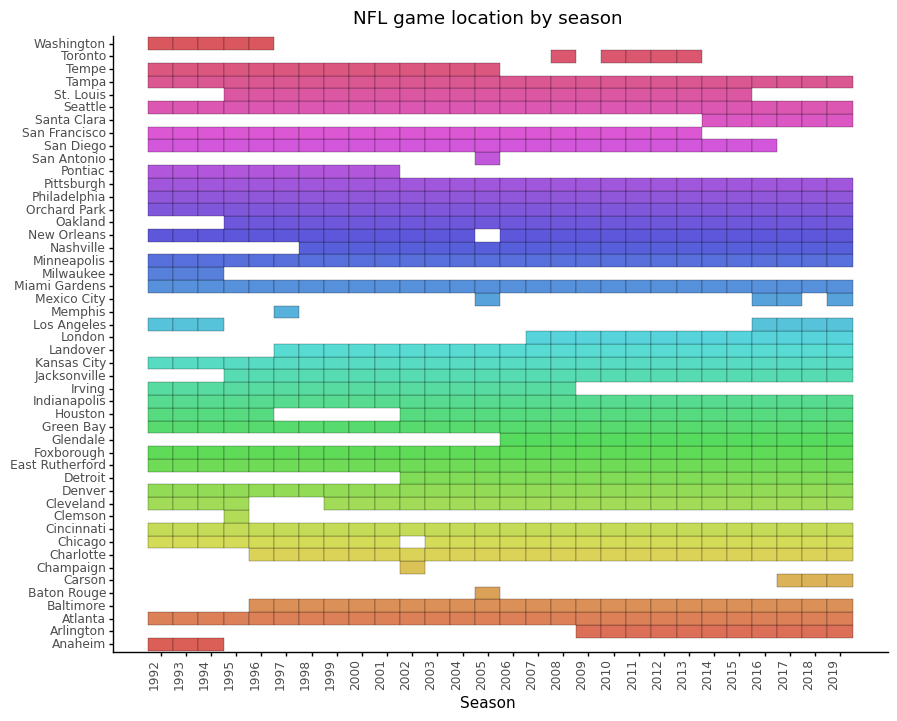
\includegraphics[width=\linewidth]{../09_figures/plot_city.png} 
    \caption{Cities where NFL games were held between the 1992 and 2019 seasons}
    \label{fig:city}%
\end{figure}

\subsubsection{Outliers}

When examining the training data set, I noticed a few outliers in the set of home field advantage feature variables. Figure \ref{fig:hfa} shows a scatter plot between  the \textit{Miles\_traveled} \textit{Time\_rest\_days} variables.
\begin{figure}[H]%
\centering
   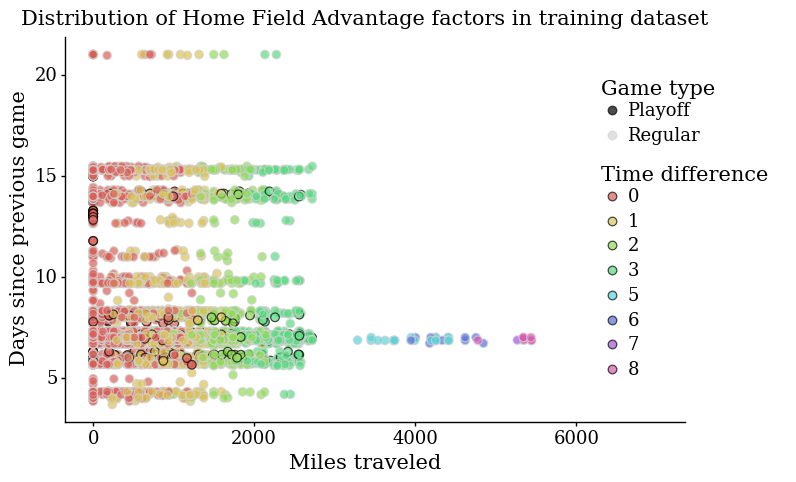
\includegraphics[width=0.75\linewidth]{../09_figures/plot_hfa.png} 
    \caption{Distribution of Home Field Advantage factors in training dataset}
    \label{fig:hfa}%
\end{figure}

The outliers in Miles traveled can be easily explained - every year since 2007, at least one game is held in London as part of the NFL International Series \citep{int}. International travels also explains the outliers in time zone differences.

The outliers in days between games is a bit more puzzling. Initially, I had assume that these were from top seeds in the playoff who got to skip a first-round bye, but I was wrong. After examining the training data, I learned that the outliers came from the synthetic way I was filling in the missingness for the \textit{Time\_rest\_days} variable described earlier in section \ref{missing}. All the outliers came from 2001. Due to the one-week postponement in week 2 after the 9/11 attack, the longest ``bye'' a team had that season was 3-weeks long. As I apply the season's longest bye week to every team's time rest for week 1, this outliers multiplied. This is a flaw in the data that I choose to accept.


\subsubsection{Rating a team}
I use PFR's Offensive Simple Rating System (OSRS) and Defensive Simple Rating System (DSRS) to rate a team's overall quality in the season. Figure \ref{fig:srs} shows the distribution of the variables in the training data. These variables measure a team strengths' relative to the average team in the regular season and centered around 0. PFR does not disclose how the OSRS and DSRS are calculated or normalized - only the overall SRS \citep{srs}, so I felt a bit uneasy using them in the model. That being said, they seem to be reasonably normally distributed and would suffice as proxy for a team's strengths and weaknesses. 
\begin{figure}[H]%
	\centering
   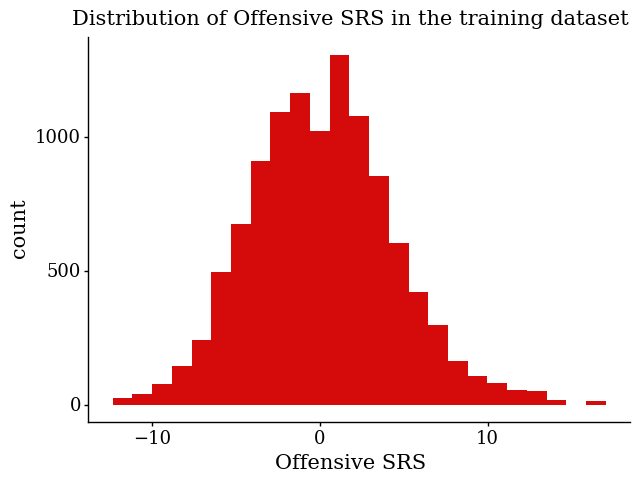
\includegraphics[width=0.49\textwidth]{../09_figures/plot_offense.png} 
   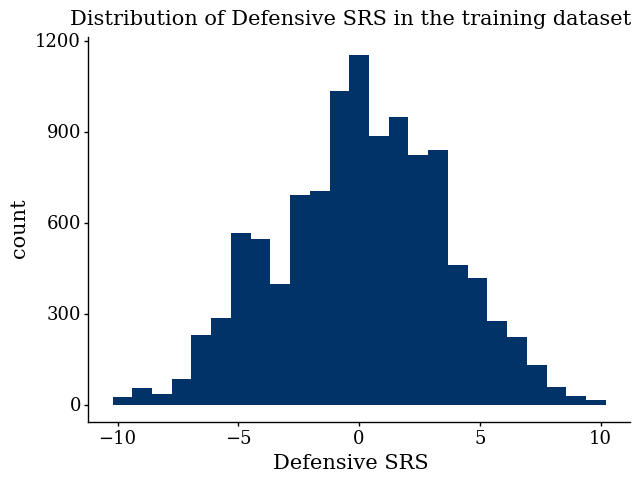
\includegraphics[width=0.49\textwidth]{../09_figures/plot_defense.png} 

    \caption{Distribution of Offensive and Defensive SRS in the training data}
    \label{fig:srs}%
\end{figure}

\subsection{Wrangling steps} \label{data1}

\subsubsection{Scraping and cleaning the scraped data} 

The most challenging part of data wrangling was to assign the correct stadium location to each of the 7292 games in the dataset. I first downloaded the HTML of the \href{https://en.wikipedia.org/wiki/Chronology_of_home_stadiums_for_current_National_Football_League_teams}{Wikipedia page with information on each time's stadium} \citep{stadium} using package requests \citep{requests} in Python, then used the package Beautiful Soup to clean up the parsed HTML to get the individual link for each stadium's URL contained in the page. With this list of URLs, I then built scrapers to retrieve the GPS coordinates for each stadium, as well as the seating capacity over the years (if the information exists). I then created a facet plot of every stadium's capacity overtime to check for missingness or strange spikes that the scraper might have missed\footnote{For example, the Seating Capacity table for the Green Bay Packers' Lambeau Field \citep{lambeau} does not have a datapoint for 2011 - therefore I filled it with capacity from the previous season}, then fixed them accordingly. 

At the same time, I scraped data for each season's schedule, game and attendance record from PFR using python package pandas, then concatenated the yearly tables into a long panel dataframe. The PFR data was quite clean to begin with, thus minimal effort was needed to further clean this data.

Afterwards, I merged the stadium data to each home team in the PFR dataset for every season, taking note of special circumstances where teams had to play at a ``home'' stadium that's not their main stadium - either due to participation in planned events\footnote{NFL International Series in the UK and Mexico \citep{int}, Bills Toronto Series in \citep{bills} }, mid-season stadium moves\footnote{For example, in 2005 the St. Louis Rams had 2 Home stadiums - Busch Memorial Stadium for the first 4 home games, and Trans World Dome for the remainder of the season \citep{rams}.}   or due to other unforeseen circumstances\footnote{For example, the New Orleans Saints played the entire 2005 season in alternate ``home'' stadiums because the Superdome suffered extensive damage due to Hurricane Katrina \citep{bills}.}. I manually fixed this part of the merged data, using raw data that I had already scraped.  

Additionally, since the data on PFR is only for regular season games, I scraped game records, schedule, location and attendance data for playoff games from Wikipedia, using techniques similar to ones described above. Finally, I merged all the data together. This dataset is set up in a wide format where each row contains information for a unique game, along with both teams' scores, ratings, as well as their respective home stadium.
\subsubsection{Setting up the dyad}

After merging the cleaned into a wide panel, I moved onto transforming it into a dyadic dataset. I created this dataset by making a mirrored copy of the wide data described above, switching the columns with information for one team with the other. Finally, I concatenated the original and mirrored data set together, and dropped the excessive columns and renamed the remaining columns accordingly. 

Finally, I calculated the \textit{Miles\_traveled} variable using the Great-Circle distance between the GPS coordinates of Team\_A's Home stadium and the stadium the game is being played at with methods described by \cite{distance}, as well as the time rest each time has between 2 consecutive games on the schedule using pandas' timedelta function. The final dyadic dataset is set up so that 2 consecutive rows make up a dyad representing one game. The team-specific information in each vector (such as miles traveled, time rest, season overall offensive rating, etc.) contains information for Team\_A in that row. This dyadic dataset is the data on which I train my models.

Finally, I split it into a training and a test dataset, with the test dataset containing 25\% of the rows in the full dataset.


\section{Analysis}

After setting up the dyad, I ran the data through a pipeline with 4 classifiers: K-nearest neighbor, Gaussian Naive-Bayesian, Decision Tree, and Random Forest, and set tuning parameters for them. Aside from the built-in MinMax scaler using sklearn API \citep{sklearn_api}, I did not do further pre-processing of my data, as I think the outliers in the feature variables such as miles traveled are important in understanding the away team's disadvantage. 

The model that ``won out'' in the pipeline is a Random Forest model with a max depth of 7, max features of 7, and 500 estimators. When using this model to predict whether it made correct predictions in the training data itself, it received an Area Under Curve (AUC) score of 0.779 and Accuracy score of 0.707. 

The AUC score of the model on the test dataset is 0.705 and the Accuracy score is 0.645. Figure \ref{fig:roc} shows the Receiving Operating Characteristic Curve illustrating the model's false positive rate and true positive rate. As a coin flip would have an AUC score of 0.5, so the black-box model does a little better than random, but not impressively so. However, the information we learn from which variable is more important in making the prediction is useful in our understanding of home field advantage, which I will discuss in more details in the next section. 

\begin{figure}[H]%
	\centering
   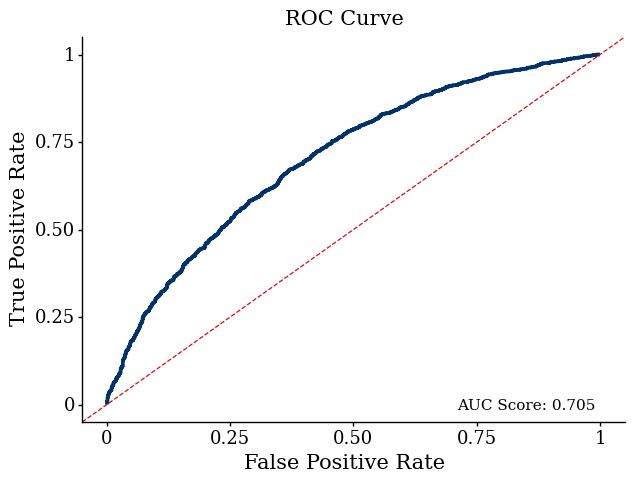
\includegraphics[width=0.5\linewidth]{../09_figures/plot_roc.png} 
    \caption{Receiver Operating Characteristic Curve}
    \label{fig:roc}%
\end{figure}

\section{Results}

Figure \ref{fig:vi} ranks the importance of the feature variables in the Random Forest model. For obvious reasons, a team's ORSR and DSRS are the 2 most important variables in whether it wins a game or not. More interesting is the next 2 important variables: \textit{Miles\_traveled} and \textit{Attendance\_pct}.

\begin{figure}[H]%
	\centering
   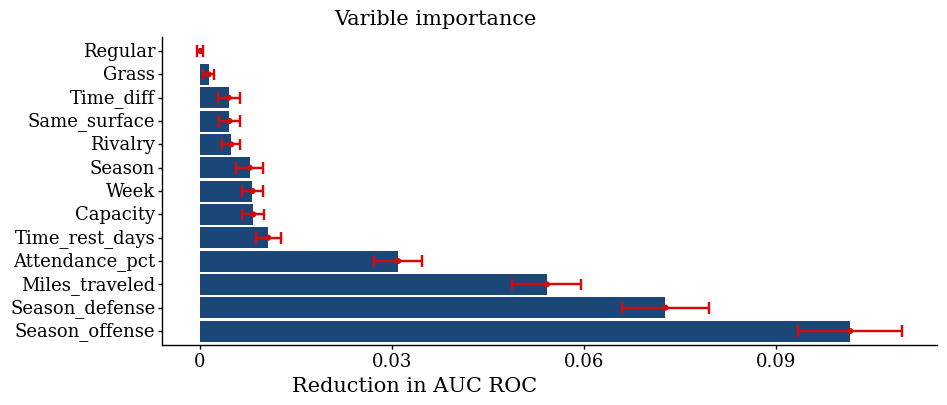
\includegraphics[width=0.8\linewidth]{../09_figures/plot_vi.png} 
    \caption{Variable importance}
    \label{fig:vi}%
\end{figure}


The Partial dependency plots in Figure \ref{fig:pdp} shows an obvious decrease in probability of winning between a team that had to travel versus one that didn't. Attendance percentage in the stadium seems to play a role in predicting a team's Win as well. Interestingly, the number of days a team gets to rest did not. 

\begin{figure}[H]%
	\centering
   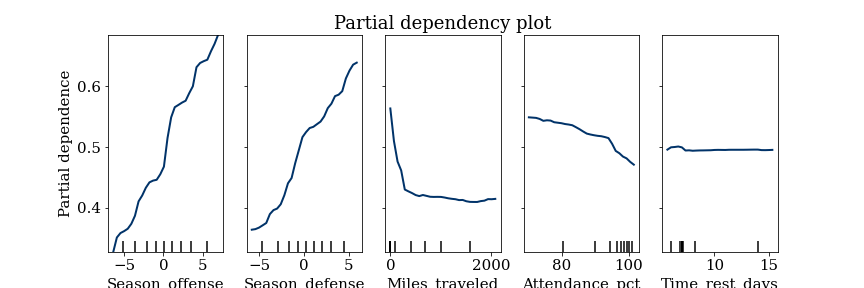
\includegraphics[width=0.8\textwidth]{../09_figures/plot_pdp.png} 
    \caption{Partial Dependency Plot (PDP)}
    \label{fig:pdp}%
\end{figure}

Figure \ref{fig:hainter} shows the interaction between \textit{Miles\_traveled} and \textit{Attendance\_pct} in predicting the outcome. The model predicts that a home team who didn't have to travel (thus \textit{Miles\_traveled} = 0) with a packed stadium will win more than teams that had to travel. Interestingly, international travels (the last column in the grid) don't seem to present much of a disadvantage, as both teams had to travel, but domestic long-distance travels do.
\begin{figure}[H]%
	\centering
   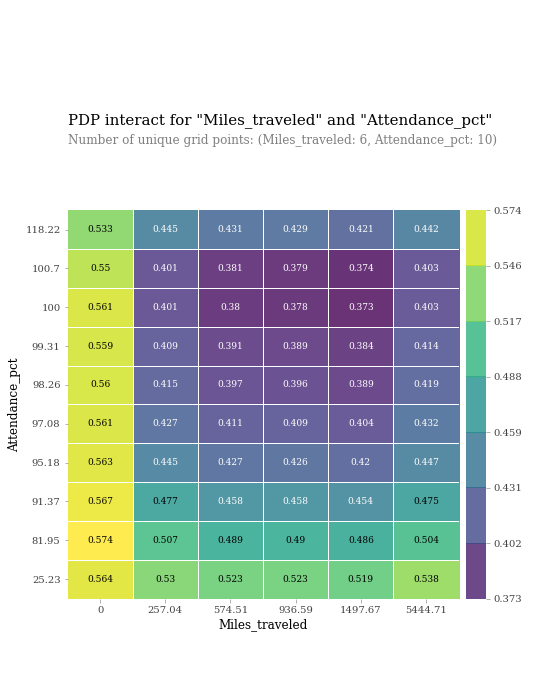
\includegraphics[width=0.5\linewidth]{../09_figures/home_attendance.png} 
    \caption{PDP interact for Miles traveled and Attendance percentage}
    \label{fig:hainter}%
\end{figure}

Figure \ref{fig:ice} shows that distance travel does have a negative impact on a team's win probability. There does seem to be heterogeneity in this - for obvious reasons, because a team's defense and offense matter more to the outcome than distance traveled.

\begin{figure}[H]%
	\centering
   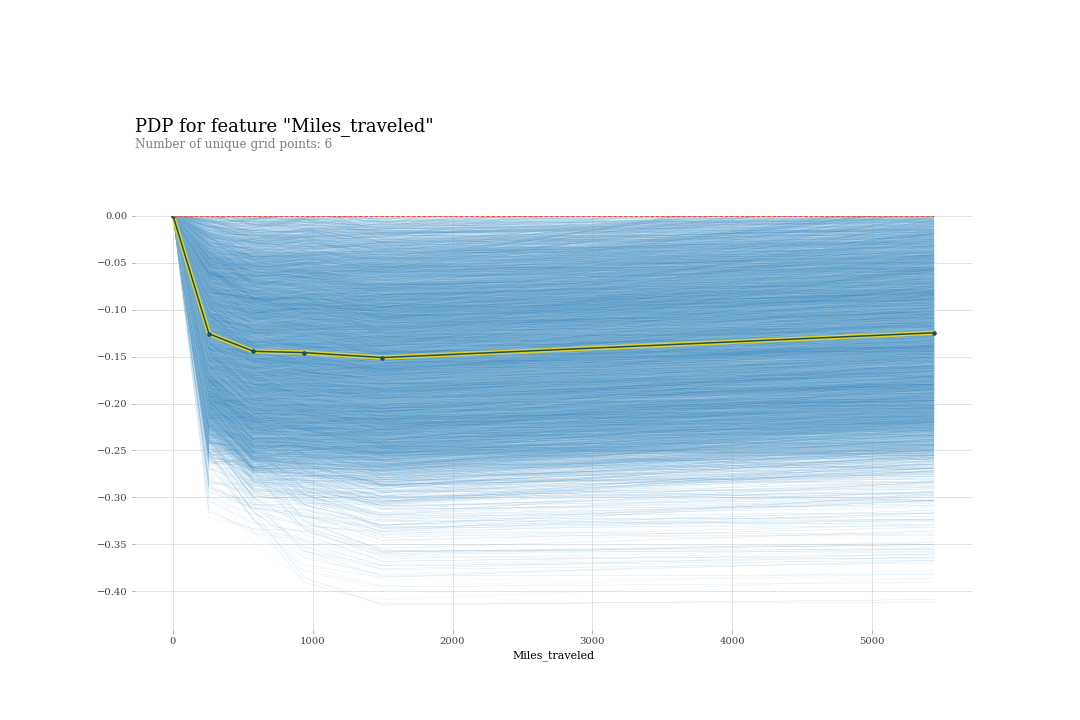
\includegraphics[width=0.5\linewidth]{../09_figures/ice_plot.png} 
    \caption{Ice plot for Mile traveled}
    \label{fig:ice}%
\end{figure}


Because the best predictor came from a Random Forest model - a black-box model that's not easily interpretable, I created a global surrogate model to interpret the result. The decision tree surrogate in Figure \ref{fig:tree} has an $R^2$ of 0.77, which means that the decision tree model explains 77\% of the behavior of the Random Forest model. This decision tree helps us understand some of the splittings that went into the black-box model in predicting a team's win. 

\begin{figure}[H]%
\hspace*{-4.5cm}
   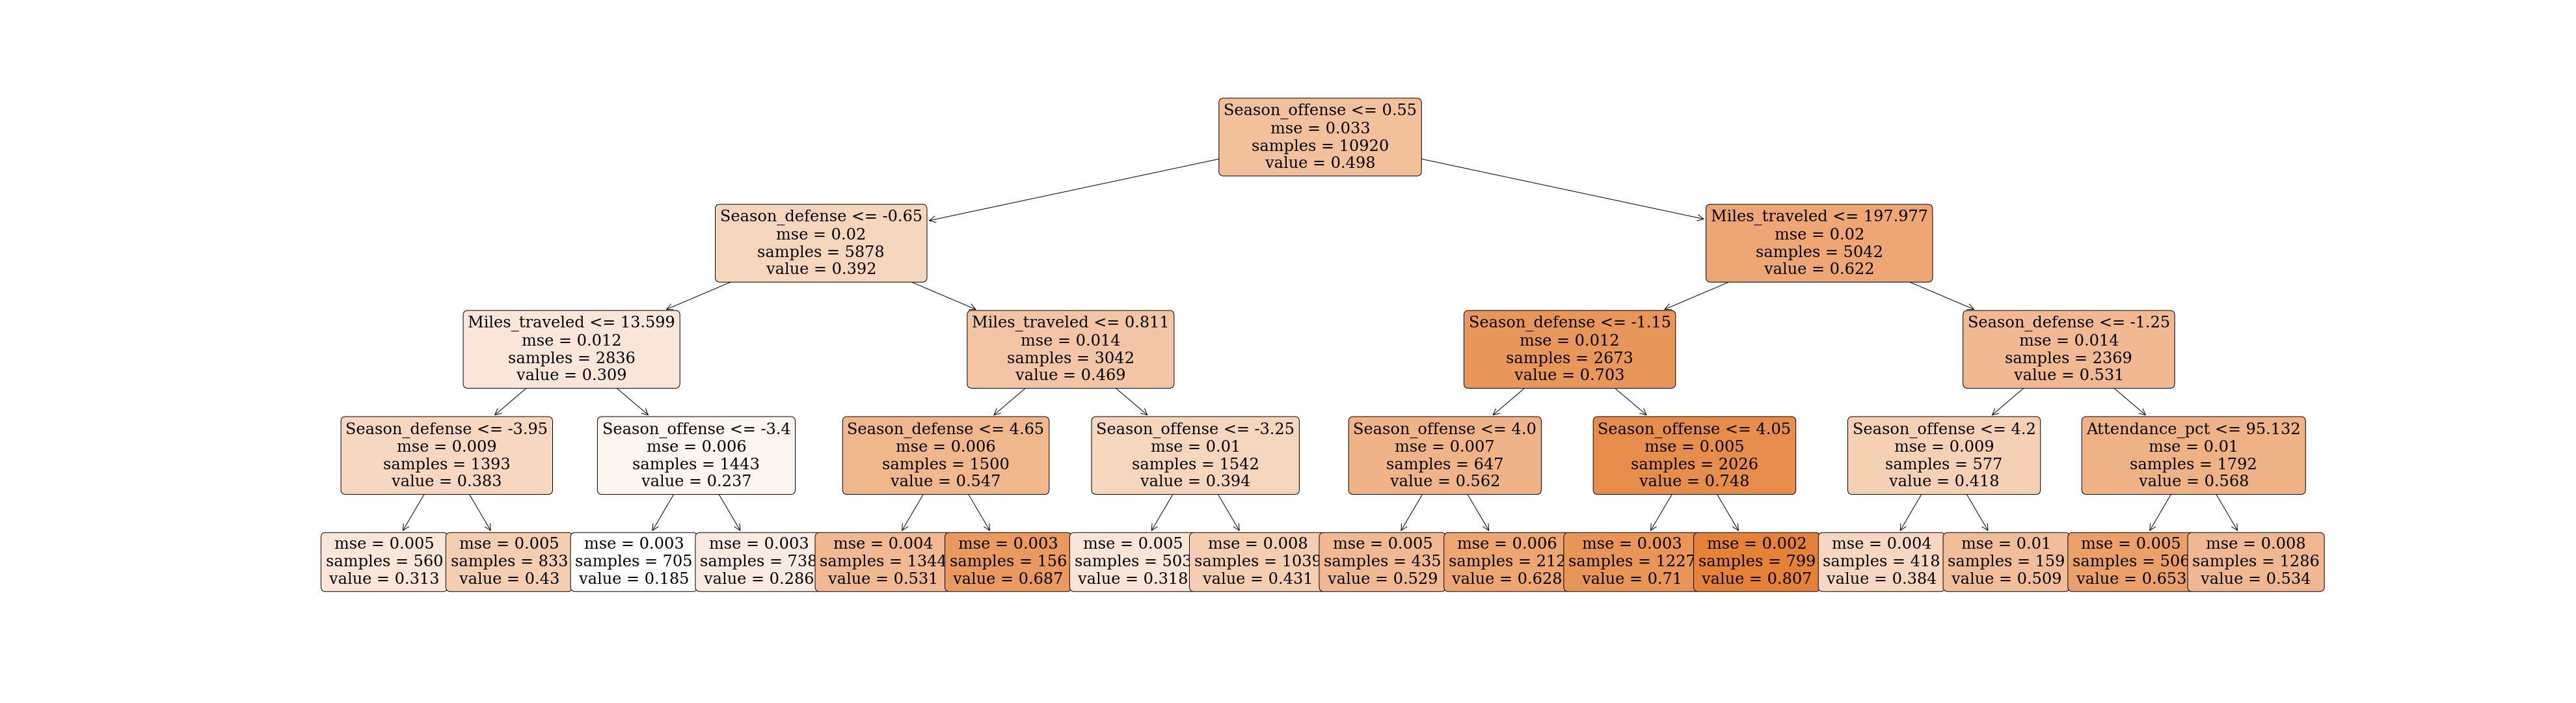
\includegraphics[width=1.5\textwidth]{../09_figures/decision_tree.png} 
    \caption{Global Surrogate Model}
    \label{fig:tree}%
\end{figure}

Out of all the feature variables, distance traveled seem to be the most likely explanation for a team's home field advantage in my model. Home teams win because they did not have to travel, and the more domestic travel a team has to do for a game, the less likely they'll win. 

\section{Further discussion}

Overall, I consider the project a moderate success. Data wrangling took the bulk of the time I spent in this project, but I learned a lot from it. I am happy that I seem to find some indication that distance travel matters more to home field advantage than crowd noise, rest time and timezone difference. 

If given more time, I would have liked to tinker more with the pre-processing steps to try to get a better accuracy score. I would also be interested to learn how the model would on games in the 2020 season - as fans attendance doesn't seem to matter as much as distance traveled (those poor Seahawks!)



\bibliography{nguyen_chau_final_project}
\bibliographystyle{apalike}



\end{document}
